
%%%%%%%%%%%%%%%
%%%      CHAPTER      %%%
%%%%%%%%%%%%%%%

\chapter{Introduction}
\label{ch:general_introduction:introduction}

%%%%%%%%%%%%%%%%%%%%%%%%%%%%%%%%%%%%%%%%%
%%%%%%%%%%%%%%%%%%%%%%%%%%%%%%%%%%%%%%%%%

\section{The limits of the modern synthesis}
\label{sec:general_introduction:introduction:darwin_limits}

Variation and selection are at the core of evolution \citep{darwin-1859}. In theory, these two mechanisms are sufficient to engage a process of Darwinian evolution, where differences in reproduction and survival rates---summarized by the concept of \textbf{fitness}---lead to the ``survival of the fittest'' \citep{spencer-1864}. During the XX\textsuperscript{th} century, the modern synthesis has been developed to rise this mechanism as the central paradigm of biology, merging C. Darwin's and G. Mendel's theories \citep{huxley-1942} (Fig. \ref{fig:general_introduction:introduction:fig1}). Variation and selection are also exploited in other fields such as evolutionary optimization algorithms. However, while the modern synthesis mostly focused on molecular evolution, at the level of the \textbf{genotype} (by attributing a fitness to an allele segregating in the population for example), selection actually plays on the \textbf{phenotype} of an organism \citep{lande-1976}. Despite the attempt of quantitative genetics to link phenotypic variability with genetic mutations, the relationship between the genotype and the phenotype, known as the \textbf{genotype-to-phenotype map} \citep{alberch-1991}, is far from being understood, and classical models of evolution are unable to explain the most integrated properties of living organisms, \textit{e.g.}, phenotypic innovations or major transitions \citep{smith-szathmary-1997}. Three main reasons could be invoked to explain the apparent failure of modern synthesis to model the most complex evolutionary outcomes:

\begin{figure}[!h]
\centering
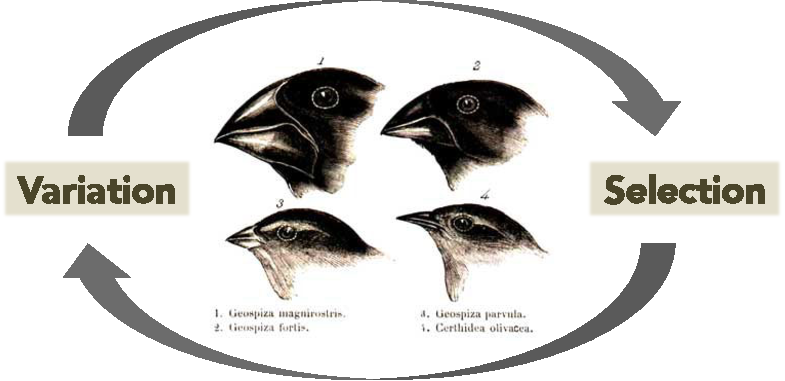
\includegraphics[width=0.6\textwidth]{generalintroduction_introduction_fig1.pdf}
\caption[Variation and selection at the heart of Darwinian evolution.]{{\bf Variation and selection at the heart of Darwinian evolution.} As symbolically represented by the Darwin finches, whose beaks are adapted to various sizes and shapes of seeds, variation and selection are at the heart of Darwinian evolution, a theoretical basis to the modern synthesis.}
\label{fig:general_introduction:introduction:fig1}
\end{figure}

\paragraph{$\bullet$ Biotic systems process information.}
In the early 1970's, Paulien Hogeweg and Ben Hesper coined the term ``bioinformatics'' to design the study of ``informatic processes in biotic systems'' \citep{hogeweg-hesper-1978,hogeweg-1978}. Even if the term has later been distorted to refer to biological data analysis, an important idea was released: according to P. Hogeweg, ``\textit{it seemed to us that one of the defining properties of life was information processing in its various forms, e.g., information accumulation during evolution, information transmission from DNA to intra and intercellular processes, and the interpretation of such information at multiple levels}'' \citep{hogeweg-2011}. Indeed, an essential property of living species seems to be their ability to accumulate information from past environments, on the long-term. By ``learning'' about past environmental features, species can ``react'' to new environments, by enhancing their \textbf{evolvability} (\textit{e.g.}, by increasing mutation rates, or favoring mutations in a specific region of their genome, ...), or their \textbf{robustness} (\textit{e.g.}, by evolving DNA repair mechanisms, or by buffering genetic variations through the regulation network, ...). During the last decades, this property of evolution received a lot of interest, and is often referred as \textbf{evolution of evolvability}\footnote{The concept of information accumulation and ``evolution learning'' is also a concern of the \textbf{extended evolutionary synthesis}, an attempt to extend the modern synthesis \citep{laland-et-al-2015,watson-szathmary-2016}.}.

\paragraph{$\bullet$ Evolution acts at multiple levels.}
In 2003, Paulien Hogeweg and Nabuto Takeuchi noticed that: ``\textit{although there has been much discussion on what is the appropriate level on which Darwinian selection operates, we now know that in many cases the interesting features arise through the occurrence of multiple levels of selection which act in concordance and/or in conflict}'' \citep{hogeweg-and-takeuchi-2003}. While the definition of ``level'' is the source of a classical debate in biology\footnote{See \cite{banzhaf-et-al-2016} for a discussion on the notion of ``biological level''.}, one would hardly disagree that life takes place on multiple physical and time scales. A living organism is composed of one or more cells, each containing a cytoplasm with numerous and complex structures, DNA, RNA, proteins and so on. Each organism interacts with its environment and with other organisms. Populations of organisms modify their environment, creating new selective pressures, and various species interact together, directly or indirectly. Life on earth thus scales from molecules to entire ecosystems, all of these structures interacting and evolving in concert. Here, a question rises about how to model such a complex system. Nobody pretends to be able to forecast the weather by only simulating a set of gas molecules under brownian motion. With such a low-scale modeling, important properties of weather, such as gravity and Coriolis forces, temperature gradients or day/night cycles will never emerge from the model. This is quite similar in evolutionary biology: a gene-centered model will not be able to produce the most integrated properties of evolution, simply because there is no support in the model for it \citep{banzhaf-et-al-2016}. To do so, \textbf{multi-level models} are needed.

\paragraph{$\bullet$ Interesting properties of evolution emerge with second-order selection.}
According to \cite{tenaillon-et-al-2001}, the Darwinian view of evolution needs a refinement to explain its ``complex dynamic aspects''. More than just a selection for better adaptation to a specific environment, \textbf{second-order selection}, or \textbf{indirect selection} \citep{kirschner-gerhart-1998,reisinger-miikkulainen-2006}, acts on the regulation of the processes of adaptation to any new environment \citep{pennisi-1998}. Some survival strategies could not evolve without second-order selection, such as evolution of mutation rates and mutators \citep{denamur-matic-2006}, or evolution of bet-hedging \citep{beaumont-et-al-2009} for example. Second-order selection is also responsible for the emergence of important processes discussed just above, such as information accumulation in biotic systems.

Finally, as shown in Figure \ref{fig:general_introduction:introduction:fig2}, long-term evolution and second-order selection led to the emergence of many mechanisms observed in living systems, at all the biological organization levels. These mechanisms directly control the variability of organisms, and are themselves under selection. Hence, we can expect that living organisms, more than being adapted to their environment, \textbf{are adapted to evolve}. \cite{hindre-et-al-2012} coined the term \textbf{evolution of evolution} (EvoEvo) to refer to this evolutionary process.

\begin{figure}[!h]
\centering
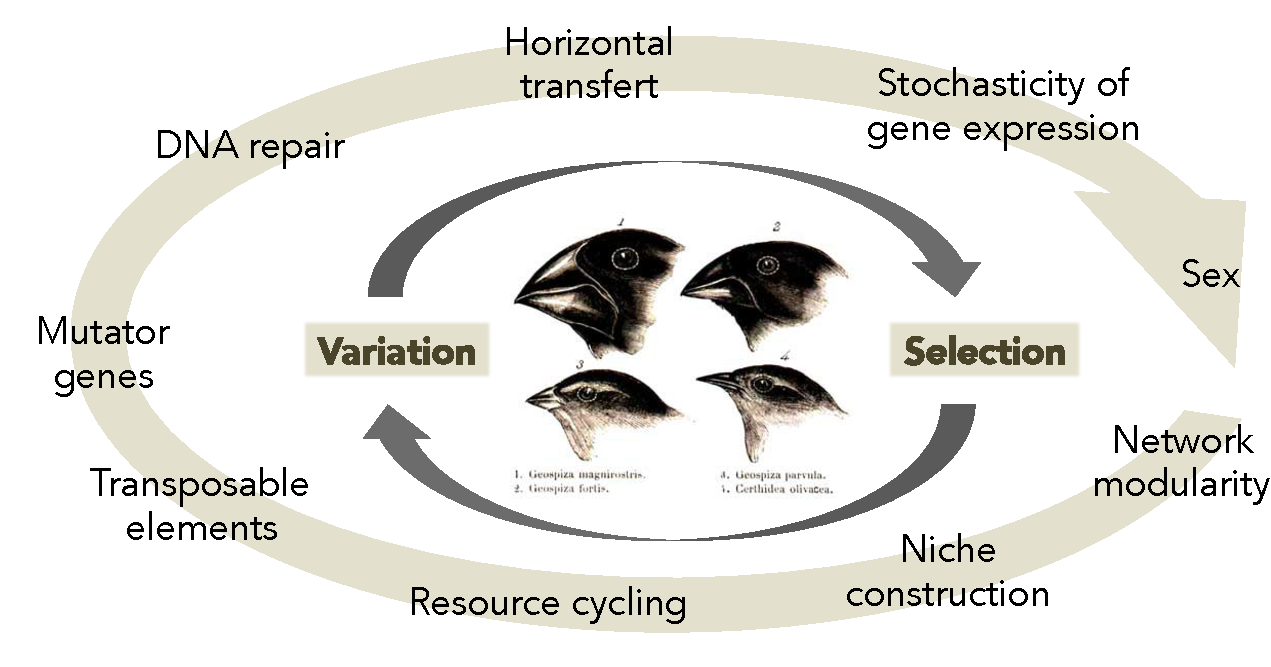
\includegraphics[width=1\textwidth]{generalintroduction_introduction_fig2.pdf}
\caption[Long-term evolution leads to evolution of evolution.]{{\bf Long-term evolution leads to evolution of evolution.} On the long-term, living organisms have evolved different mechanisms (DNA repair, horizontal transfer, sex, and so on) that control their own variability. However, these mechanisms are themselves under selection, implying that the basic mechanisms of evolution are therefore themselves evolving, a process called evolution of evolution, or EvoEvo.}
\label{fig:general_introduction:introduction:fig2}
\end{figure}

%%%%%%%%%%%%%%%%%%%%%%%%%%%%%%%%%%%%%%%%%%
%%%%%%%%%%%%%%%%%%%%%%%%%%%%%%%%%%%%%%%%%%

\section{What is evolution of evolution?}
\label{sec:general_introduction:introduction:what_is_evoevo}

By evolving, living organisms permanently adapt to rarely stable and sometimes unpredictable environments. Moreover, organisms constantly modify their environment, by interacting with it and by evolving, thus generating complex and challenging conditions. While higher eukaryotes have evolved complex sensori-motor systems to plastically adapt to environmental variations, micro-organisms (that represent more than an half of the biomass on earth) do not have such complex sensoring abilities. However, they are surprisingly efficient to adapt to their environment by simply ... evolving. Many experimental studies demonstrated that bacteria and viruses are able to adapt to new environments in only a few tens of generations \citep{rainey-travisano-1998,zhang-et-al-2011}. Hence, micro-organisms are excellent candidates to study evolution of evolution \citep{hindre-et-al-2012}.

EvoEvo encompasses the evolution of four essential evolutionary properties: \textbf{variability}, \textbf{evolvability}, \textbf{robustness}, and \textbf{open-endedness}. While the notions of evolvability and robustness pervaded theoretical evolutionary biology during the last decades, the concept of open-endedness is more familiar to computational scientists. However, it is strongly related to \textbf{phenotypic innovations} and \textbf{major transitions} \citep{smith-szathmary-1997}, two important concepts in evolutionary biology.

%%%%%%%%%%%%%%%%%%%%%%%%%%

\subsection{Variability}
Variability is the ability to generate new phenotypes. It is a necessary condition for any evolutionary process to take place. A lot of biological mechanisms have been identified that produce and/or control variability:
\begin{enumerate}
% GENETIC VARIABILITY
\item[\textbf{(1)}] \textbf{Genetic variability.}  For historical reasons, genetic variability has been widely studied during the XX\textsuperscript{th} century, and a variety of mutational events altering genomes have been identified (point mutations, small insertions and deletions, large rearrangements, horizontal transfers, gene amplifications, ...). Many mechanisms are known to modify the rate at which these mutation events occur in the genome, locally or globally, as reviewed in \cite{ryall-et-al-2012}. For example, when \textbf{contingency loci}---localized on small portions of the genome---are mutated, mutation rates are locally increased. Another example is \textbf{mutations in DNA repair or maintenance genes}, that can lead to hyper-mutator strains, which have constitutively elevated mutation rates. In some conditions, these strains can be positively selected and favor adaptation \citep{tenaillon-et-al-1999,denamur-matic-2006}. As a last example, \textbf{transient changes in the expression level of DNA repair and maintenance genes} allow for rapid mutation rates increase in case of environmental stress \citep{foster-2007};
% PHENOTYPIC PLASTICITY
\item[\textbf{(2)}] \textbf{Phenotypic plasticity.}
According to \cite{stearns-1989}, phenotypic plasticity refers to phenotypic variability in response to the environment. Micro-organisms own genetic regulation networks, able to sense their environment. Evolution can shape these regulation networks such that one genotype can produce many phenotypes as a function of an environmental signal (the reaction norm). When one genotype produces several discrete phenotypes depending on the environmental signal, we speak about \textbf{polyphenism}. When one genotype produces a single phenotype, whatever the environmental variations, we speak about \textbf{environmental canalization}, one source of evolutionary robustness \citep{waddington-1942};
% EPIGENETIC INHERITANCE
\item[\textbf{(3)}] \textbf{Transgenerational epigenetic inheritance.}
According to \cite{veening-et-al-2008}, epigenetic inheritance refers to any transmission of a cellular state from one generation to another without genome modification. A classical example of this mechanism is DNA methylation or acetylation \citep{avery-2006}.
For example, the agouti yellow mouse phenotype is due to the unmethylation of the retrotransposon gene \textit{Avy}, inserted upstream of \textit{agouti} gene. Agouti yellow mices have yellow coat and suffer obesity. It appeared that unmethylated sequences are transmissible from one generation to the other via the gametes, without modification of the genotype.
% PHENOTYPIC STOCHASTICITY
\item[\textbf{(4)}] \textbf{Phenotypic stochasticity.}
Finally, the stochastic fluctuations of the phenotype (or phenotypic noise) are an important source of variability \citep{symmons-and-raj-2016}. Phenotypic noise is mainly due to the inherent stochastic nature of biochemical reactions inner the cell, because of the low number of implicated molecules and thermodynamic fluctuations. An example is \textbf{stochastic gene expression} (SGE). SGE has an important role in genetic regulation and the emergence of interesting phenotypic properties such as stochastic switching \citep{acar-et-al-2008,tsuru-et-al-2011}. Stochastic fluctuations are of primary importance in some survival strategies, such as bet-hedging \citep{veening-et-al-2008}, as reviewed in details by \cite{dejong-et-al-2011}. The evolution of phenotypic noise will be studied in part \ref{part1} of this manuscript.
\end{enumerate}

All these mechanisms being themselves under selection, we can expect that variability---and thus evolution---can evolve.

%%%%%%%%%%%%%%%%%%%%%%%%%%

\subsection{Evolvability and robustness}
The question of the evolution of evolvability and its relationship with the evolution of robustness has received important contributions in the last years. However, the question is still open. While the term evolvability has been used in different ways \citep{wagner-2013}, it is usually defined as \textbf{the ability to increase the proportion of beneficial mutations}, while robustness is defined as \textbf{the ability to withstand mutations without losing fitness}. Both mechanisms has been shown to evolve, mainly in numerical simulations (see \textit{e.g.} \citealt{bedau-packard-2003,elena-sanjuan-2008,crombach-hogeweg-2008,beslon-et-al-2010a}). Demonstrating evolution of evolvability or robustness experimentally is much more difficult since it necessitates to perform experimental evolution experiments, which are long and costly (see \textit{e.g.} \citealt{elena-and-lenski-2003}).

At first sight, evolvability and robustness seem to be antagonistic. An evolvable organism should not be robust, and a robust organism should not be evolvable. However, the remarkable ability of Darwinian evolution to generate sophisticated emergent properties is demonstrated here. Indeed, evolvability has an important role in \textbf{innovation}: a biological system is evolvable if it can acquire novel functions through genetic change that increase fitness \citep{wagner-2005}. However, and counter-intuitively, robustness and \textbf{neutral mutations} also play a key role in the innovation process, because they allow to explore the phenotypic space while the fitness of the organism remains constant. By exploring the neutral landscape of an organism, neutral mutations promote future innovation.

This mechanism has nicely been represented by \cite{wagner-2008b} (Fig. \ref{fig:general_introduction:introduction:fig3}). Let's consider a network of all possible genotypes of an organism, each node being a genotype, linked to accessible other genotypes by single mutations. A fitness is attributed to each genotype. Some mutations are neutral, meaning that they link two genotypes with the same fitness, negative (if they decrease the fitness), or positive. A positive mutation can also be an innovation (the acquisition of a novel function with a beneficial fitness value, as discussed later in this introduction). For a robust organism, many mutations are neutral, such that evolution consists to travel in the neutral genotype network. Robust organisms can thus explore vast regions of the genotype network with no consequence on their fitness, and access new genotypes not accessible otherwise. As metaphorically stated by A. Wagner:
\begin{quote}
Perhaps the most compact way to express this problem is with an analogy from politics: evolving populations need to be both ``conservative'' and ``progressive'' at the same time \citep{wagner-2012}.
\end{quote}

\begin{figure}[!h]
\centering
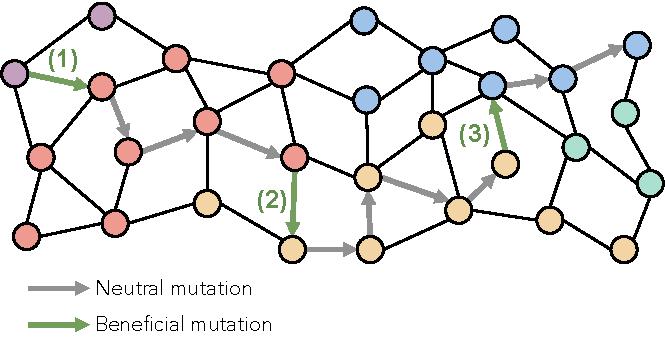
\includegraphics[width=0.7\textwidth]{generalintroduction_introduction_fig3.pdf}
\caption[Evolution on the genotype network for a robust organism.]{{\bf Evolution on the genotype network for a robust organism.} Each genotype is represented by a node, colored according to its fitness. Single mutations linking genotypes together generate a network, explored by evolving populations of organisms. The successive fixed mutations are represented by a path on this network. Beneficial mutations are represented by green arrows, while neutral ones are represented by grey arrows. Here, the evolutive path is composed by long successive travelling sessions on the neutral network, punctuated with three beneficial mutations (inspired from \citealt{wagner-2008b})}
\label{fig:general_introduction:introduction:fig3}
\end{figure}

%%%%%%%%%%%%%%%%%%%%%%%%%%

\subsection{Open-endedness}
The notion of open-endedness has been extensively discussed in \cite{banzhaf-et-al-2016}. Often defined as the ability to continuously produce novelty and/or complexity, open-endedness is a quite fuzzy notion. Considered as an important modeling challenge in the field of artificial life, the term is almost unknown in theoretical biology. Indeed, this recent concept still needs to be properly defined. According to \cite{banzhaf-et-al-2016}, open-endedness is essentially a \textbf{modeling concept}, and can refer to the capacity of a model to generate ``novelty''. \cite{banzhaf-et-al-2016} identified three types of novelties, depending on model capabilities: \textbf{variation}, \textbf{innovation} and \textbf{emergence}:

\begin{enumerate}
\item[\textbf{(1)}] \textbf{Variation.} A variation is defined here as a change to the values of a variable, or an instance in the model. This means that variations are simply the exploration of the predefined space of the model (``\textit{novelty in the model}'', \citealt{banzhaf-et-al-2016}). This definition could correspond to the notion of variability presented above;
\item[\textbf{(2)}] \textbf{Innovation.} An innovation is a change to the model itself. Hence, an innovation modifies the space in which variation can operate (``\textit{novelty that changes the model}'', \citealt{banzhaf-et-al-2016}). This definition could correspond to the notion of innovation discussed above;
\item[\textbf{(3)}] \textbf{Emergence.} Emergence is a change to the ``meta-model''. Indeed, a model is the instantiation of a conceptual model, defining types of objects and their relationships (``\textit{novelty that changes the meta-model}'', \citealt{banzhaf-et-al-2016}). This idea is exemplified by \cite{andrews-et-al-2011}: collective behavior (\textit{e.g.} collective bird fly) is often modeled by a class of individual-based models known as flocking or boids models \citep{reynolds-1987}. It is first needed to define the behavior of the boids (to define the agents), and then to collect individual positions (to collect data) in order to detect flockness (to measure the data). Then, a meta-model of a flocking model is the association of the concepts of agent, data and measure \citep{andrews-et-al-2011}. The notion of emergence directly refers to \textbf{major transitions}. According to \cite{smith-szathmary-1997}, a major transition occurs when ``\textit{entities that were capable of independent replication before the transition can only replicate as parts of a large unit after it}''. The comprehension of this property of living organisms is an important challenge for evolutionary biologists.
\end{enumerate}

We see that the concepts of variability, evolvability, robustness and open-endedness are intertwined in a complex way. Their evolution also require interdependencies between many mechanisms and properties, at multiple levels of biological organization.

%%%%%%%%%%%%%%%%%%%%%%%%%%%%%%%%%%%%%%%%%%%%%%%%
%%%%%%%%%%%%%%%%%%%%%%%%%%%%%%%%%%%%%%%%%%%%%%%%
\section{Capturing the whole spectrum of EvoEvo, or the necessity to build multi-level models}
\label{sec:general_introduction:introduction:evoevo_is_multilevel}

%%%%%%%%%%%%%%%%%%%%%%%%%%

\subsection{Modeling choices and the experimental method}
Building a model is a tough task, since modeling choices depend on the scientific question, but also on the kind of desired output (consciously or not) and maybe on some intuition. On this point, the modeling work presented in this manuscript has been largely influenced by the approach of the INRIA-Beagle team, in particular the works of \cite{knibbe-2007} and \cite{beslon-2008} on the modeling of complex biological systems.
A model is always false, and implies unavoidable assumptions, simplifications and shortcuts \citep{banzhaf-et-al-2016}. But more than that, when a model is correctly used to produce a new hypothesis or theory, this hypothesis or theory should acquire its own existence, independently from the model \citep{grimm-1999}. In this sense, the model is useful to generate new ideas, but should then disappear in their shadow \citep{beslon-2008}.

According to \cite{servedio-et-al-2014}, in evolutionary research, as in many other fields, some models are conceived to test the logic of verbal explanations of a theory, in the same way that empirical data is used to test scientific hypotheses. To build such a \textbf{proof-of-concept model}, we should follow the four steps of the \textbf{experimental method} promoted by Claude Bernard: \textbf{(i)} First, observe the nature and build hypotheses. \textbf{(ii)} Then, pick assumptions and build a model. \textbf{(iii)} Third, analyze the model, and finally \textbf{(iv)} evaluate new hypotheses and propose new directions, closing the loop (Fig. \ref{fig:general_introduction:introduction:fig4}). Even if the reality of scientific modeling has been shown to be more complex (the four steps are often interconnected, and even self-connected, such that building a model consist in navigating between them, \citealt{chalmers-1990,beslon-2008}), we should stick to this ``best practice'' guideline as much as possible. The hardiest task (but also the most exciting) probably consists in picking the right assumptions and build the model.

There is no well-defined guideline to pick the modeling assumptions, and to adjust the complexity of the model. However, depending on the scientific question, the model must at least represent the objects of interest, and their interactions. Regarding the study of EvoEvo, two important theoretical objects summarize the relationship between an evolving organism and its environment: \textbf{the genotype-to-phenotype map}, and the \textbf{fitness landscape}:

\begin{enumerate}
\item[\textbf{(1)}] \textbf{The genotype-to-phenotype map.}
The phenotype of an organism results from a complex and non-linear cascade of developmental, physiological and regulatory processes, summarized by the concept of genotype-to-phenotype map. According to the central dogma of molecular biology \citep{crick-1958}, the development of an organism reflects the flow of information from the genetic sequence to the phenotype. As such, the genotype-to-phenotype map is an object that represents all the functions of an organism (transcription, translation, regulation, protein folding, metabolism, environmental sensing, and so on). Hence, the genotype-to-phenotype map is generally a very complex object, an important condition to the evolution of evolution, as discussed above.
\item[\textbf{(2)}] \textbf{The fitness landscape.}
The fitness landscape is considered as one of the most important concepts in theoretical evolutionary biology. The fitness landscape projects the space of all possible genotypes, or phenotypes of a population of organisms in the space of fitness values, usually through a fitness function. Firstly used by \cite{wright-1932}, the fitness landscape is at the heart of historical models of evolution, such as \textbf{Fisher's geometric model} \citep{fisher-1930} or \textbf{NK-fitness landscapes model} \citep{kauffman-levin-1987}. The latter has been used to show how the complexity of a landscape influences the course of an evolutionary process \citep{correia-fonseca-2007}. The former will be presented in detail in part \ref{part1} of this manuscript. Often represented by a smooth function (\textit{e.g.}, a Gaussian-shaped function in Fisher's geometric model), the fitness landscape of living organisms is probably a much more complex, fluctuating and highly dimensional landscape (as discussed below).
\end{enumerate}

\begin{figure}[!ht]
\centering
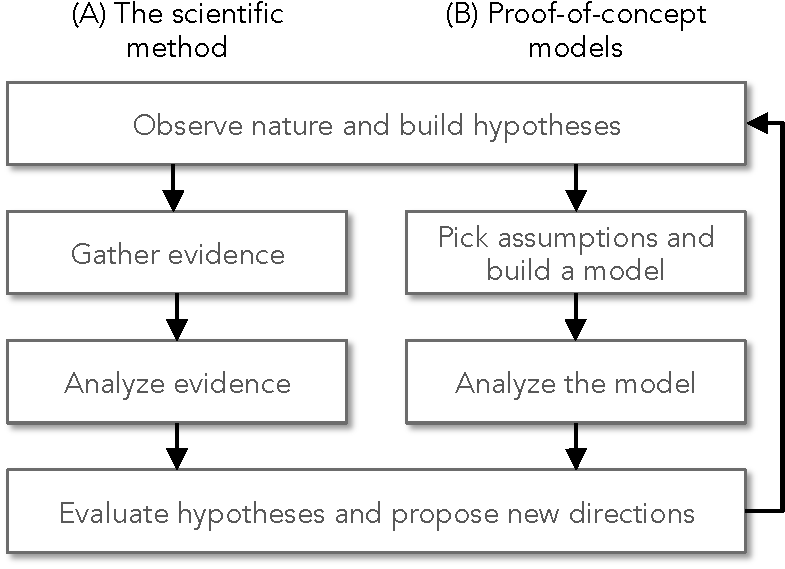
\includegraphics[width=0.6\textwidth]{generalintroduction_introduction_fig4.pdf}
\caption[Proof-of-concept modeling and the scientific method.]{{\bf Proof-of-concept modeling and the scientific method.} This flowchart shows the steps in the scientific process, with a parallel between the scientific method, as defined by C. Bernard, and proof-of-concept modeling methodology. (A) The main steps of the scientific method. (B) The steps of proof-of-concept modeling (inspired from \citealt{servedio-et-al-2014}).}
\label{fig:general_introduction:introduction:fig4}
\end{figure}

%%%%%%%%%%%%%%%%%%%%%%%%%%

\subsection{The necessity of multi-level modeling of evolution}
Computational models have been used to study evolution since the beginning of the 1990's \citep{adami-2006}. However, since then, most computational models used a partial representation of the genotype-to-phenotype map, generally in a fixed, predefined, fitness landscape. Yet, fitness is the result of the interaction of all the biological structures of an organism, including its interactions with the environment. Similarly, the variability/robustness/evolvability/open-endedness of the phenotype is the result of the interaction of variability/robustness/evolvability/open-endedness of all the biological structures of an organism, including its interactions with its environment. Furthermore, these properties are co-dependent and they may interact in a cooperative or competitive way (\textit{e.g.}, evolving chaperone proteins reduce phenotypic variability, thereby increasing robustness). Moreover, both the genotype-to-phenotype map and the fitness landscape are very likely to change during the course of evolution. That is why a computational model of EvoEvo must be multi-level, including the main organization levels of the genotype-to-phenotype map and the fitness landscape (genome, transcription network, metabolic network, phenotype, fitness, population, environment, and so on).

First, the genotype-to-phenotype map has long been considered as a one-directional and deterministic process, the genetic information flowing from the genotype to the phenotype. However, the development of living organisms is a non-deterministic process, depending on many molecular mechanisms that are fundamentally stochastic, as demonstrated by the stochastic nature of gene expression \citep{elowitz-et-al-2002}. Thus, one genotype can lead to several random phenotypes, and this stochastic variability can itself evolve through the genotype-to-phenotype map, as discussed in part \ref{part1} of this manuscript. Moreover, the information can flow back from the phenotype to the genotype (\textit{e.g.}, thanks to RNA interference, genetic regulation, or environment influence). Altogether, these mechanisms make the genotype-to-phenotype map of an organism a very complex object to analyze, generating non-intuitive situations through evolution of evolution.

Second, the fitness landscape of living organisms is much more complex than suggested in early models of evolutionary biology. The fitness of an organism depends on its environment. However, organisms constantly interact with it (including other organisms), such that the fitness landscape is constantly fluctuating, triggering complex evolutionary outcomes, such that co-evolution, niche construction, resource cycling, and ultimately major transitions. Some authors use the concept of \textbf{fitness seascape} to render the effect of fluctuating fitness landscapes on evolution \citep{mustonen-lassig-2009}.

As a whole, we see that the genotype-to-phenotype map and the fitness landscape form a complex system, which cannot be modeled statically as it is the case in classical mathematical representations \citep{fisher-1930,kauffman-levin-1987} (even the number of dimensions in the fitness landscape and in the genotype-to-phenotype map are evolvable). Moreover, both the genotype-to-phenotype map and the fitness landscape interact through evolution, a condition for evolution of evolution. For these reasons, a model of evolution of evolution should necessarily include complex, multi-layered and evolvable genotype-to-phenotype map and fitness landscape. Such a model will incorporate a large set of parameters and its study is likely to be very difficult. But as a compensation, it will give rise to new hypotheses and predictions, impossible to obtain with previous models.

%%%%%%%%%%%%%%%%%%%%%%%%%%

\subsection{But ...}
Based on the previous arguments, one could argue that our modeling approach should be exclusively a computational multi-scale approach, in the hope to observe the most complex features of EvoEvo; it would be foolish to do so. \textbf{(i)} The first reason is that history of theoretical evolutionary biology demonstrated the importance of mathematical models to understand evolution. From mendelian genetics to population genetics, quantitative genetics, coalescence theory, and so on, mathematical models remain the most powerful---and convincing---scientific tools. \textbf{(ii)} The second reason is that when the intuition of an hypothesis or a theory is acquired by the exploitation of a computational model of evolution, the best practice would be to derivate the mathematical equations representing the phenomenon in a more abstract way, and provide a robust mathematical analysis, if possible. This is for example the case for {\aevol} model \citep{knibbe-et-al-2007a} (presented below): in {\aevol}, a strong correlation between the genome size of bacterial-like digital organisms and their mutation rates has been identified. This observation has further been generalized with a more abstract mathematical model \citep{fischer-et-al-2014}.
\textbf{(iii)} The third reason is more practical: if some properties of EvoEvo can be studied with mathematical models, there is no reason not to do it \citep{peck-2004}. The approach used in this manuscript mostly results from this last reason. We decided to have a complementary approach, anchored in the modeling practice of the INRIA-Beagle team, using both sustainable mathematical and complex multi-scaled and individual-based approaches, as exemplified in the next parts of this manuscript.

%%%%%%%%%%%%%%%%%%%%%%%%%%%%%%%%%%%%%
%%%%%%%%%%%%%%%%%%%%%%%%%%%%%%%%%%%%%
\section{State of the art}
\label{sec:general_introduction:introduction:state_of_the_art}

We have seen above that the study of EvoEvo requires the use of a variety of models, including mathematical and multi-scaled individual-based approaches. In both cases, many models, with sometimes a long history behind them, already allowed to largely highlight the evolutive interactions between the genotype-to-phenotype map and the fitness landscape. Two modeling approaches will be presented below, and then be used as a basis to decipher some aspects of EvoEvo: \textbf{(i) Fisher's geometric model}, an historical mathematical model of the genetic theory of adaptation, and \textbf{(ii) digital genetics} formalism, that led to an experimental method in evolutionary modeling: \textbf{in silico experimental evolution}.

%%%%%%%%%%%%%%%%%%%%%%%%%%

\subsection{Fisher's geometric model of adaptation}

Fisher's geometric model (FGM, \citealt{fisher-1930}) has a long and interesting history (reviewed in \citealt{orr-2005,tenaillon-2014}), and received renewed interest in the last decades. According to \cite{tenaillon-2014}, a reason is that behind its apparent simplicity and limited number of parameters, FGM integrates a full model of mutations and epistatic interactions, with surprising emergent properties.

In FGM, each phenotypic character of an organism is represented by an axis in a Cartesian coordinate system. R.A. Fisher used the term \textbf{phenotypic complexity} to refer to the dimensionality $n$ of this space. Let's define the phenotype of an organism with $n$ characters by a point $\boldsymbol{z} = (z_1, z_2, ..., z_n)^T$ ($T$ being the matrix transposition operator). The fitness $W(\boldsymbol{z})$ of this organism is then determined by its distance to the fitness optimum $\boldsymbol{z_{opt}}$, such that:
\begin{equation}
W(\boldsymbol{z}) = exp \left[ -(\boldsymbol{z}-\boldsymbol{z_{opt}})^T \boldsymbol{\Sigma}^{-1} (\boldsymbol{z}-\boldsymbol{z_{opt}})\right]
\end{equation}
where $\boldsymbol{\Sigma}$ denotes a $n \times n$ positive-definite and symmetrical matrix defining the shape of the fitness landscape. For the sake of simplicity, an isotropic fitness landscape is usually assumed, meaning that fitness varies independently and in the same proportion for all characters. The origin of the coordinate system is also used as the fitness optimum ($\boldsymbol{z_{opt}} = \boldsymbol{0})$, such that the fitness function is reduced to a simple Gaussian-shaped function:
\begin{equation}
W(d) = \exp \left[ -\dfrac{d^2}{2} \right]
\label{eq:fitness_function}
\end{equation}
with $d = \lVert \boldsymbol{z} \rVert$ the euclidean distance of the phenotype $\boldsymbol{z}$ from the fitness optimum. Mutations are represented by a random vector $\boldsymbol{r} = (r_1, r_2, ..., r_n)^T$ moving the ancestral phenotype $\boldsymbol{z}$ to its offspring $\boldsymbol{z'}$ such that $\boldsymbol{z'}=\boldsymbol{z}+\boldsymbol{r}$. The probability distribution of the mutants is often characterized by a multivariate normal distribution of the form:
\begin{equation}
p(\boldsymbol{r}) = \dfrac{1}{\sqrt{(2\pi)^n|\boldsymbol{\Sigma_r}|}} \exp \left[ -\dfrac{1}{2}\boldsymbol{r}^T \boldsymbol{\Sigma_r}^{-1} \boldsymbol{r} \right]
\end{equation}
with $\boldsymbol{\Sigma_r}$ a covariance matrix. Thus, a mutation can potentially modify every characters, a property known as the \textbf{universal pleiotropy assumption} \citep{wagner-and-zhang-2011}. Usually, initial conditions are a maladapted clonal population of asexual organisms, sitting at a certain distance from the optimum $\boldsymbol{z_{opt}}$. Then, the work consists in studying the bout of adaptation towards the optimum. FGM implies some well-known assumptions, as described in details in \cite{martin-2014}: \textbf{(i)} the distribution of all random variables have finite mean and variance and satisfy Lindeberg's conditions (the central limit theorem can be applied), \textbf{(ii)} the fitness function is twice differentiable and admits at least one non-degenerate optimum, \textbf{(iii)} mutations have mild effects on the phenotype (mutational events remain ``local''), \textbf{(iv)} each mutation potentially affect every characters (the universal pleiotropy assumption), and \textbf{(v)} the variety of mutants is very large, such that quantitative characters vary continuously (the infinite-alleles approximation).

For a given phenotype $\boldsymbol{z}$, \cite{fisher-1930} demonstrated that the probability $P_a(x)$ that a random mutation of a given phenotypic size $s$ is favorable is $1-\Phi(x)$, where $\Phi$ is the cumulative distribution function of a standard normal random variable, and $x$ is a standardized mutational size $x = s\sqrt{n}/(2d)$. $n$ is the number of characters and $d = \lVert \boldsymbol{z} \rVert$ is the euclidean distance to the optimum. As shown in Figure \ref{fig:general_introduction:introduction:fig5}A, this probability quickly decreases with the mutational size.

R.A. Fisher also suggested that organisms may pay a cost for the complexity of their phenotype (the complexity being defined here as the number of characters $n$ under selection), because the probability to fix a beneficial mutation of a certain size literally vanishes when the number of characters increases \citep{orr-2000}. In consequence, only mutations with a very small size should segregate in a population. R.A. Fisher argued that his result was a demonstration of a \textbf{micro-mutationism} view of evolution, populations evolving smoothly by very little steps. However, R.A. Fisher omitted to consider that mutations occur in populations of finite size. As later demonstrated by M. Kimura with the neutral theory of evolution, new mutations appearing in a population have a significative chance to be lost at random, especially when their beneficial value is low. Thus, according to the cost of complexity and the effects of genetic drift, we should expect that only mutations of an intermediate size would segregate in an evolving population. Finally, as discussed by \cite{orr-2005}, evolution towards a fitness optimum cannot be reduced to the study of a single mutational event. When the entire boot of adaptation towards the fitness optimum is scrutinized in FGM, it appears that the size of fixed mutations depends on the distance from the optimum: very few large mutations are usually necessary to approach the fitness optimum, the remaining distance being filled with many small mutations, as shown in Figure \ref{fig:general_introduction:introduction:fig5}B.

\begin{figure}[!ht]
\centering
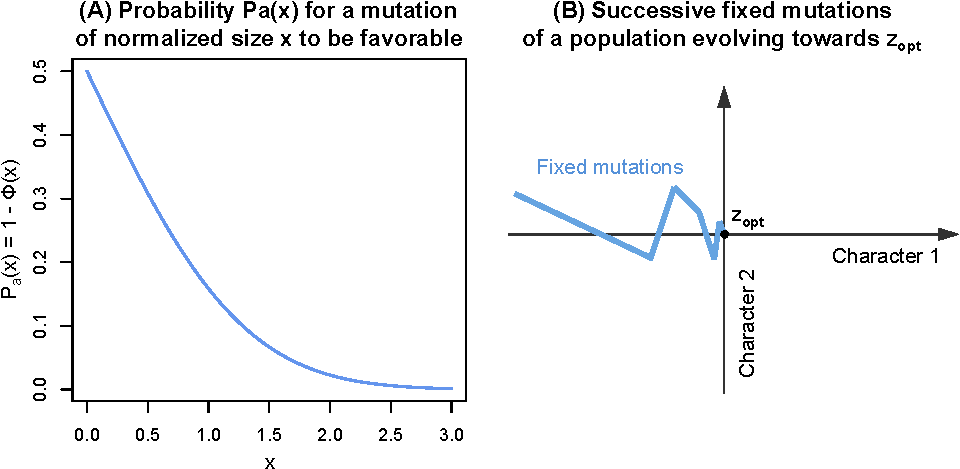
\includegraphics[width=0.9\textwidth]{generalintroduction_introduction_fig5.pdf}
\caption[The beneficial value of a mutation in FGM depends on its size.]{{\bf The beneficial value of a mutation in FGM depends on its size.}
\textbf{(A)} The probability $P_a(x)$ for a mutation of normalized size $x = s\sqrt{n}/(2d)$ (with $n$ the number of characters, and $d = \lVert \boldsymbol{z} \rVert$ the euclidean distance from the fitness optimum) to be favorable is $P_a(x) = 1-\phi(x)$ (blue curve). \textbf{(B)} When a population evolves towards the fitness optimum $\boldsymbol{z_{opt}}$, a few number of large mutations are usually sufficient to approach $\boldsymbol{z_{opt}}$. Then, a lot of small mutations are necessary to reduce this distance to zero, as shown in blue (inspired from \citealt{orr-2005}).}
\label{fig:general_introduction:introduction:fig5}
\end{figure}

%%%%%%%%%%%%%%%%%%%%%%%%%%

\subsection{In silico experimental evolution: a tool to study evolution}
\textit{In silico} experimental evolution \citep{hindre-et-al-2012,mozhayskiy-tagkopoulos-2013,batut-et-al-2013} is an approach based on the usage of individual-based models to evolve \textbf{digital organisms} in a computer, a field known as \textbf{digital genetics}. In digital genetics models \citep{adami-2006}, organisms are modeled by data-structures representing their genotype. The kind of structure used depends on the studied level(s) of organization (numerical vectors, binary sequences, regulation network, ...) and the formalism used to develop the model (reviewed in \citealt{mozhayskiy-tagkopoulos-2013,hindre-et-al-2012}). As discussed in part \ref{part2} of this manuscript, the development of an \textit{in silico} model of evolution needs some ``ingredients''. The minimum requirement is the \textbf{evolutionary engine} enabling the data-structures to reproduce, mutate and be selected depending on a fitness function. Many digital genetics models have been proposed in the literature, Avida being the best known \citep{wilke-et-al-2001,adami-2006}. However, only a few models are able to efficiently address questions related to evolution of evolution, in particular because most formalisms impose that the structure of organisms and the fitness landscape are fixed over time.

The increasing number of parameters and the computational and time resources needed to run multi-scale individual-based simulations forbid an exhaustive and rigorous exploration of the parameters and state spaces of the system, as it could be the case for Fisher's geometric model for example.
Hence, an \textbf{experimental approach} is needed to study this kind of models. According to \cite{peck-2004}, complex simulation models should be explored with the same experimental and statistics tools used for real systems:
\begin{quote}
Simulations are experimental systems. Their complexity can make them closer cousins in complexity to nature itself than to simple analytic models, but with a powerful advantage over the real world: the modeler has complete control of the system \citep{peck-2004}.
\end{quote}
In evolutionary biology, the experimental method that consists in studying evolving organisms is \textbf{experimental evolution}. In experimental evolution, fast replicating micro-organisms (\textit{e.g.}, bacteria or viruses) are being evolved in controlled environments for thousands of generations \citep{philippe-2007}. It is then possible to recover precisely the evolutionary history of lab strains by reviving frozen samples \citep{elena-and-lenski-2003}. However, despite its explanatory and statistical power, experimental evolution remains a long and costly process. \textbf{In silico experimental evolution} (ISEE) consists in mimicking this process with digital organisms \citep{hindre-et-al-2012,mozhayskiy-tagkopoulos-2013,batut-et-al-2013}, as shown in Figure \ref{fig:general_introduction:introduction:fig6}: ancestral microbial (or digital) populations are evolved in controlled environments and regularly frozen (or saved in a backup), independent repetitions are made, and frozen populations can be revived (or reloaded in memory) to perform competition experiments and other analyses. ISEE approach while be exemplified in the part \ref{part2} of this manuscript.

\begin{figure}[!ht]
\centering
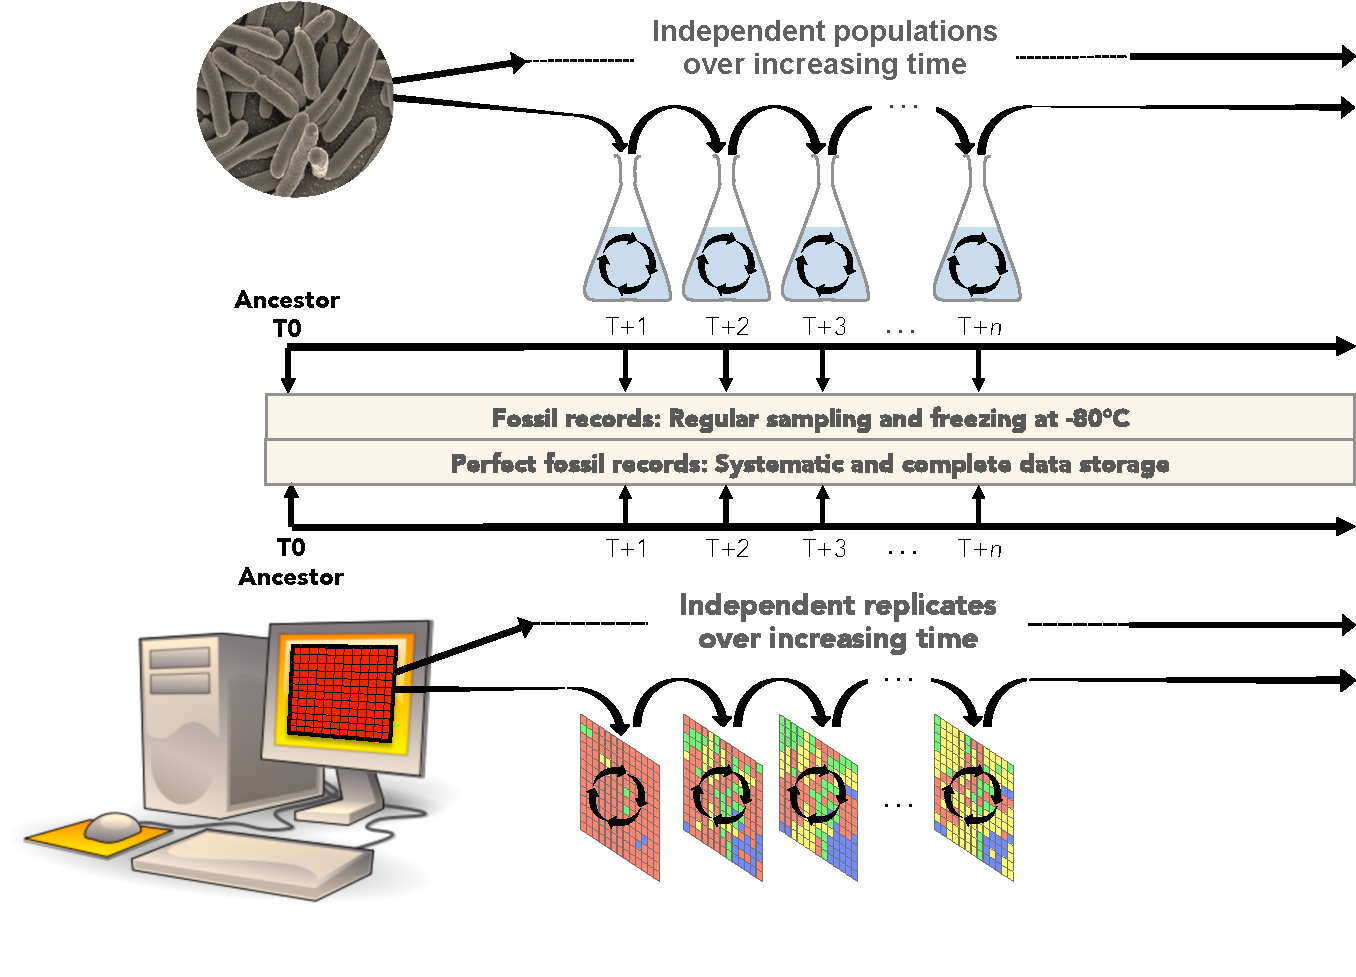
\includegraphics[width=1\textwidth]{generalintroduction_introduction_fig6.pdf}
\caption[In vivo and in silico evolution experiments.]{{\bf In vivo and in silico evolution experiments.}
Ancetral real micro-organisms (top) and digital organisms (bottom) are propagated in controlled environments, in a laboratory or in a computer respectively. Wet or digital populations are regularly frozen, or saved in backups, respectively and can be revived or reloaded at any time.
Many replicate populations can be independently evolved from a common ancestor T0 (inspired from \citealt{hindre-et-al-2012}).}
\label{fig:general_introduction:introduction:fig6}
\end{figure}

Two formalisms have recently been used to develop computational models allowing for \textit{in silico} experimental evolution. \cite{knibbe-et-al-2007a,knibbe-et-al-2007b} used the \textbf{sequence-of-nucleotides} formalism to develop {\aevol} software. With this model, the authors showed that indirect selection could select specific genetic and network structures depending on the mutational and selective pressures \citep{knibbe-et-al-2007b,beslon-et-al-2010a,beslon-et-al-2010b}. In parallel, \cite{crombach-hogeweg-2008} developed the \textbf{pearls-on-a-string} formalism and used it to show that, in time-varying environments, regulation networks, metabolic networks and species networks can acquire structures that increase the evolvability of the organisms \citep{crombach-hogeweg-2007,crombach-hogeweg-2008,crombach-hogeweg-2009}. These two formalisms are described in the next sections.

%%%%%%%%%%%%%%%%%%%%%%%%%%

\subsection{The sequence-of-nucleotides formalism}
In the sequence-of-nucleotides formalism, the genome is a variable-length string of characters. Predefined signal sequences, analogous to promoters, terminators or start/stop codons, are used to detect genes. Therefore, mutational processes, such as point mutations, small insertions and deletions, or large rearrangements can be simulated in a realistic manner \citep{hindre-et-al-2012}. The sequence-of-nucleotides formalism has been successfully used to study \textit{e.g.}, the evolution of non-coding DNA and the genes number \citep{knibbe-et-al-2007b}, the evolution of the size and topology of gene networks \citep{kuo-et-al-2006,beslon-et-al-2010a}, gene network interference \citep{mattiussi-floreano-2007,marbach-et-al-2009}, the evolution of ``public good'' production \citep{frenoy-et-al-2013}, and the reduction of genome size in some species \citep{batut-et-al-2013}.

Here, we will focus on the {\aevol} software \citep{knibbe-et-al-2007a}, because we will get inspired from its genome and genetic regulation representations in the following. In {\aevol}, each digital organism owns a circular, double-stranded chromosome (Fig. \ref{fig:general_introduction:introduction:fig7}a) that is actually a string of binary nucleotides, 0 being complementary of 1 and reciprocally. This chromosome contains coding sequences (genes) separated by non-coding regions. Each coding sequence is detected by a transcription-translation process and decoded into a ``protein'' able to contribute positively or negatively to a range of abstract quantitative characters (Fig. \ref{fig:general_introduction:introduction:fig7}a). The mechanisms of transcription and translation are modeled in detail (Fig. \ref{fig:general_introduction:introduction:fig7}b,c,e), depending on a genetic code (Fig. \ref{fig:general_introduction:introduction:fig7}d). The combination of all proteins yields the value of each abstract phenotypic character (Fig. \ref{fig:general_introduction:introduction:fig7}g). Adaptation is then measured by comparing the phenotypic values to an arbitrary set of target values. The most adapted individuals have higher chances of reproduction. When a chromosome is replicated, it can undergo point mutations, small insertions and small deletions, but also large chromosomic rearrangements: duplications, large deletions, inversions, and translocations. The various types of mutations can modify existing genes, but also create new genes, delete some existing genes, modify the length of the intergenic regions, modify gene order, and so on.

\begin{figure}[!ht]
\centering
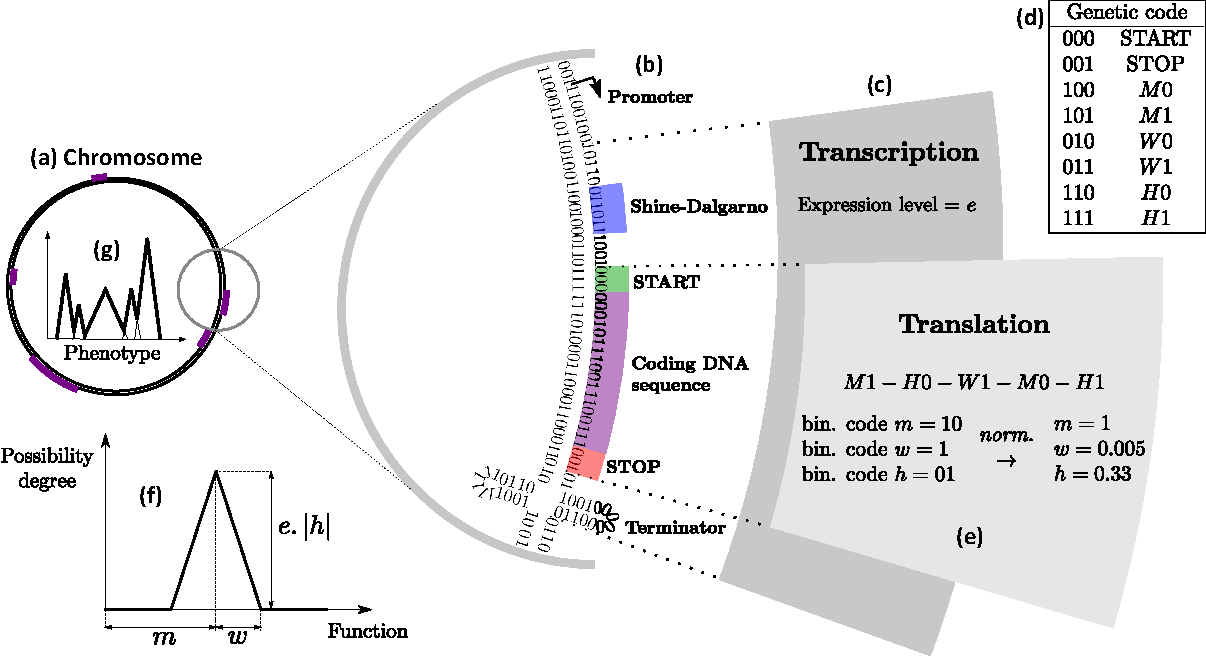
\includegraphics[width=1\textwidth]{generalintroduction_introduction_fig7.pdf}
\caption[A description of {\aevol} model.]{{\bf A description of {\aevol} model.}
In the model, each organism owns a circular double-stranded binary chromosome \textbf{(a)} along which genes are delimited by predefined signal sequences \textbf{(b)}. Promoters and terminators mark the boundaries of RNAs \textbf{(c)} within which coding sequences are in turn identified between a Shine-Dalgarno-START signal and an in-frame STOP codon. Each coding sequence is then translated into a protein sequence using a predefined genetic code \textbf{(d)}. This protein sequence is decoded as three real parameters called m, w and h \textbf{(e)}. Proteins, phenotypes and environments are represented similarly through mathematical functions that associate a level to each abstract phenotypic character in [0, 1]. The contribution of a protein is a piecewise-linear function with a triangular shape, with position $m$, half-width $w$ and height $h$ \textbf{(f)}. All proteins encoded in the chromosome are then combined to compute the phenotype \textbf{(g)}, which is compared to the environmental target to compute the fitness of the individual (inspired from \citealt{knibbe-parsons-2014}).}
\label{fig:general_introduction:introduction:fig7}
\end{figure}

{\aevol} model has been extended to include regulation of genetic expression, by adding a representation of cellular gene networks \citep{beslon-et-al-2010a}. This extended version of {\aevol}, named R-{\aevol}, is a model of prokaryotic regulation. To simulate the interactions between \textbf{transcription factors} and \textbf{promoters}, two \textbf{binding sites} are defined for each promoter. Located immediately before the promoter, the \textbf{enhancer site} increases the transcriptional activity when transcription factors bind to it. Directly following the promoter, \textbf{the operator site}, down-regulates the promoter's activity when a transcription factor binds to it. Each promoter $i$ owns a basal expression level $\beta_i$, which depends on how close its sequence is to a consensus sequence. The transcriptional activity of this promoter depends on the combined activity of the enhancer site activity $A_i$ and the operator site activity $O_i$, that read:
\begin{equation}
A_i(t) = \sum_j c_j(t)A_{ji}
\end{equation}
and:
\begin{equation}
O_i(t) = \sum_j c_j(t)O_{ji}
\end{equation}
with $A_{ji}$ (resp. $O_{ji}$) the affinity of protein $j$ for the enhancer site of the promoter $i$ (resp. for the operator site) and $c_j(t)$ the concentration of protein $j$ at time $t$.

The transcription rate $e_i(t)$ of the RNA sequence associated to the promoter $i$ is then given by the following Hill-like function:
\begin{equation}
e_i(t) = \beta_i \left( \dfrac{\theta^n}{O_i(t)^n+\theta^n} \right) \left( 1 + \left( \dfrac{1}{\beta_i}-1\right) \left( \dfrac{A_i(t)^n}{A_i(t)^n+\theta^n} \right) \right)
\end{equation}
where $n$ and $\theta$ are the two parameters defining the shape of the Hill-function. Finally, given the transcription rate, one can compute the protein concentration (for simplicity, it is assumed that the protein concentration is linearly proportional to the RNA concentration) through the following synthesis-degradation rule:
\begin{equation}
\left\{
\begin{array}{rcl}
c_i(0) & = & \beta_i/\phi\\\\
\dfrac{d c_i}{d t} & = & e_i(t) - \phi c_i(t)
\end{array}
\right.
\end{equation}
where $\phi$ is a temporal scaling constant representing the protein degradation rate. Thus, when a gene is regulated, the concentration of its product is scaled up or down depending on its transcription rate.

%%%%%%%%%%%%%%%%%%%%%%%%%%

\subsection{The pearls-on-a-string formalism}

In the pearls-on-a-string formalism, the genome is a variable-length string of ``pearls'' of different types: phenotype genes, transcription factor genes, repeats, retrotransposons, binding sites, and so on. Each pearl type can exist in a predefined number of variants. Mutational operators (point mutations, rearrangements) can modify the genes number, the order of the pearls and the regulation. The pearls-on-a-string formalism has been successfully used for the study of genome and network evolvability \citep{crombach-hogeweg-2007,crombach-hogeweg-2008}, resource processing in ecosystems \citep{crombach-hogeweg-2009}, and sympatric speciation \citep{tentussscher-hogeweg-2009}.

Recently, \cite{cuypers-hogeweg-2012} developed a multi-scale model based on the pearls-on-a-string formalism: the Virtual Cell model.
As shown on Figure \ref{fig:general_introduction:introduction:fig8}, in Virtual Cell model, digital organisms own circular genomes made of ``pearls'', encoding for five types of proteins. Organisms grow on an externally provided resource $A$ (Fig. \ref{fig:general_introduction:introduction:fig8}a), by pumping it (Fig. \ref{fig:general_introduction:introduction:fig8}b) or by passive diffusion through the cell's membrane (Fig. \ref{fig:general_introduction:introduction:fig8}c). The pumps require the consumption of an energy carrier molecule $X$, enzymatically produced from $A$ by a catabolic reaction (Fig. \ref{fig:general_introduction:introduction:fig8}d). Both $A$ and $X$ molecules are required to build end products via another enzymatic reaction (Fig. \ref{fig:general_introduction:introduction:fig8}e). Two other protein types are transcription factors that up-regulate or down-regulate the production of proteins depending on the effect of their ligands, $A$ or $X$ (Fig. \ref{fig:general_introduction:introduction:fig8}f). With their model, \cite{cuypers-hogeweg-2012} proposed that the complex genotype-to-phenotype map of digital organisms drives genome size dynamics, due to an emerging interplay between adaptation, neutrality, and evolvability, showing that genome expansion and streamlining are generic patterns of evolving systems. More recently, \cite{cuypers-et-al-2017} shown with the Virtual Cell model that depending on the frequency of environmental changes, digital organisms evolve different adaptive strategies: when the change frequency is low, evolution leads to phenotypic plasticity, while when the change is high, evolution leads to enhanced evolvability.

\begin{figure}
\centering
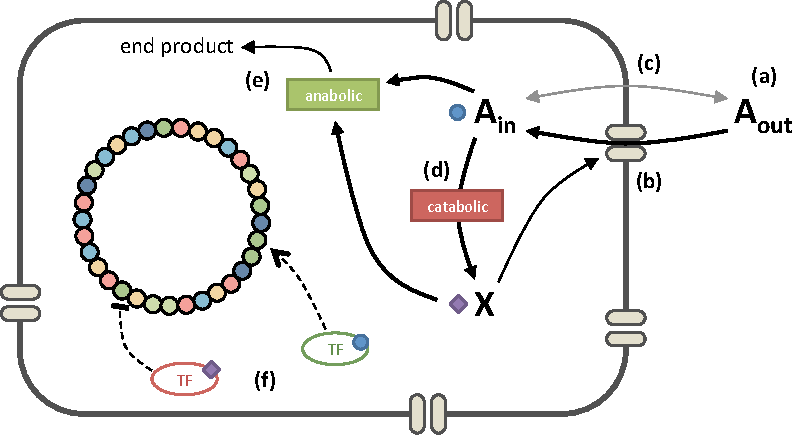
\includegraphics[width=1\textwidth]{generalintroduction_introduction_fig8.pdf}
\caption[A description of the Virtual Cell model.]{{\bf A description of the Virtual Cell model.}
In Virtual Cell model, digital organisms own circular genomes made of ``pearls'', encoding for five types of proteins. Organisms grow on an externally provided resource $A$ \textbf{(a)}, by pumping it \textbf{(b)} or by passive diffusion through the cell's membrane \textbf{(c)}. The pumps require the consumption of an energy carrier molecule $X$, enzymatically produced from $A$ by a catabolic reaction \textbf{(d)}. Both $A$ and $X$ molecules are required to build end products via another enzymatic reaction \textbf{(e)}. Two other protein types are transcription factors that up-regulate or down-regulate the production of proteins depending on the effect of their ligands, $A$ or $X$ \textbf{(f)} (inspired from \citealt{cuypers-hogeweg-2012}).}
\label{fig:general_introduction:introduction:fig8}
\end{figure}

%%%%%%%%%%%%%%%%%%%%%%%%%%%%%%%%%%%%%%%%
%%%%%%%%%%%%%%%%%%%%%%%%%%%%%%%%%%%%%%%%
\section{An attempt to merge sequence-of-nucleotides and pearls-on-a-string formalisms}
\label{sec:general_introduction:introduction:bag_of_tuples}

%%%%%%%%%%%%%%%%%%%%%%%%%%
\subsection{A common formalism: the ``bag of tuples''}

The \textbf{sequence-of-nucleotides} and the \textbf{pearls-on-a-string} formalisms have a common property: while their genomic representation (the way information is stored in the genome) differ significantly, in both formalisms, a non-ordered set of tuples is extracted from the genomic data-structure: a \textbf{bag of tuples}.

A tuple is an ordered list $(x_1,x_2,...,x_n): T_1 \times T_2 \times ... \times T_n$ with $T_i$ the ``product type'' of $x_i$ (\textit{e.g.}, $\mathbb{R}$, $\mathbb{N}$,...). In both sequence-of-nucleotides and pearls-on-a-string formalisms, the genotype-to-phenotype map is based on the extraction of an unordered set of tuples from the genotype. This set of tuples is then used to build the higher organism level in another specified space. For example, {\aevol} uses a complex and non-linear artificial genetic code to extract a set of triplets $(m,w,h) \in \mathbb{R}^3$ from a circular and double-stranded binary sequence. In pearls-on-a-string models, the genome is an unordered list of tuples. Depending on the complexity of projection operators, the evolution on the genome structure and the genotype-to-phenotype map will not be the same. In both models, the order of the tuples does not impair the fitness, but, since the tuples are encoded locally in the genome (in coding regions, or in pearls), the modification of their order on the sequence can potentially affect long-term evolution, as demonstrated in \cite{knibbe-et-al-2007a,knibbe-et-al-2007b}.
 
%%%%%%%%%%%%%%%%%%%%%%%%%%
\subsection{Bags of tuples and artificial chemistries}

When developing a new individual-based model of evolution, one important task is to define an \textbf{artificial chemistry} for this model: how to represent the various bio-molecules (DNA, RNA, proteins, metabolites, and so on) and their interactions? Artificial chemistry (AChem) is an entire field of research \citep{dittrich-2001,banzhaf-yamamoto-2015}, which is not directly in the scope of this manuscript. However, it is important to define here the most basic steps necessary to develop an AChem:

An AChem can be defined as a triplet $(S,R,A)$, where $S$ is the set of all possible molecules, $R$ is a set of reaction rules representing the interactions among the molecules, and $A$ is an algorithm describing the reaction vessel or domain and how the rules are applied to the molecules inside the vessel \citep{dittrich-2001}. The set of molecules $S = \{s_1,s_2,...,s_n\}$ can potentially be infinite. A reaction rule $r \in R$ is a chemical equation:
\begin{equation}
s_1 + s_2 + ... + s_i \rightarrow s'_1 + s'_2 + ... + s'_j
\end{equation}
With the reactants (or the substrates) on the left side, and the products on the right side. $i$ is the order of the reaction. The set of reaction rules $R$ can be defined explicitly (all possible reactions $r$ are defined and are in finite number), or implicitly. In this example, stoichiometry is 1 for all reactants, but there is no constraint on this point. The algorithm $A$ is applied on an instance of $S$, that is, a collection $P$ of molecules. The set of chemical equations $R$ can be solved with stochastic or deterministic methods, possibly adding spatial rules.

From this simple definition, two ways to define an AChem in the bag-of-tuples formalism are possible in first instance (Fig. \ref{fig:generalintroduction:introduction:fig9}):
\begin{enumerate}
\item[\textbf{(1)}] Each tuple codes for a reaction rule. In this case, each organism $i$ owns a specific set of reactions rules $R_i$, somehow carrying its own artificial chemistry. For instance, a tuple $(x_1,x_2,...,x_n)$ could define the chemical equation of order $n/2$:
\begin{equation}
s_1 + s_2 + ... + s_{\frac{n}{2}} \rightarrow s_{\frac{n}{2}+1} + s_{\frac{n}{2}+2} + ... + s_n
\end{equation}
With $x_i \equiv s_i$ (Fig. \ref{fig:generalintroduction:introduction:fig9}.1).
\item[\textbf{(2)}] Each tuple codes for a chemical species, being potentially a reactant for a subset of reactions in $R$. In this case, $R$ is defined once for the whole system, a reaction occurring only if all the reactants are present. For instance, let's consider the set of reaction rules $R$ containing the reaction:
\begin{equation}
s_i + s_j \leftrightarrow s_i . s_j
\label{eq:reaction1}
\end{equation}
And the reaction:
\begin{equation}
s_i . s_j \rightarrow s_k + s_j
\label{eq:reaction2}
\end{equation}
With $s_i, s_j, s_k \in S$, and ``.'' symbolizing a chemical bound. Thus, a singleton $x_j \equiv s_j$ (a tuple of length 1) catalyzes the enzymatic reaction:
\begin{equation}
s_i + s_j \leftrightarrow s_i . s_j \rightarrow s_k + s_j
\label{eq:reaction3}
\end{equation}
To describe more precisely the reaction, it is also possible to replace the singleton $x_i$ by a pair $(x_j, c_j)$, with $c_j = [s_j]$. With this AChem, a tuple could encode a useless compound, if no other reactant is present (Fig. \ref{fig:generalintroduction:introduction:fig9}.2).
\end{enumerate}

\begin{figure}[!ht]
\centering
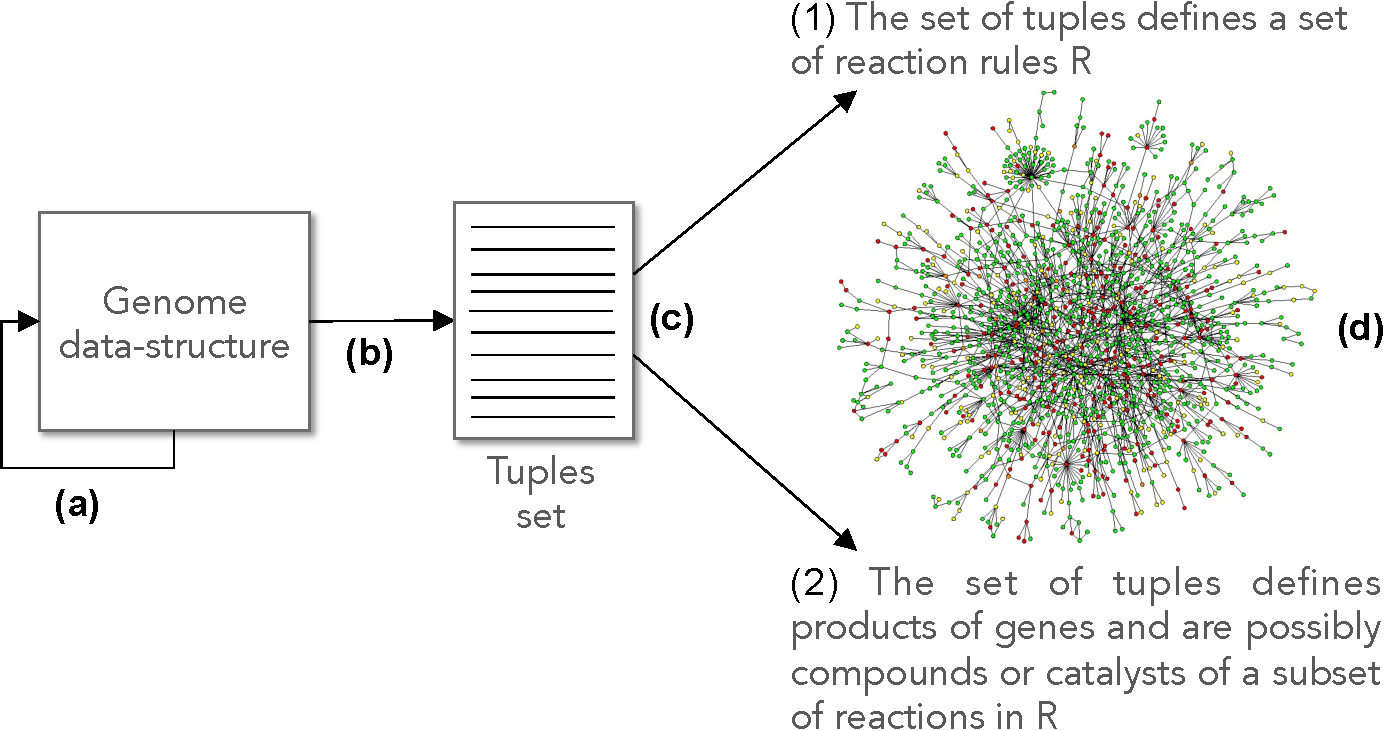
\includegraphics[width=0.7\textwidth]{generalintroduction_introduction_fig9.pdf}
\caption[A general framework for the bag-of-tuples formalism.]{{\bf A general framework for the bag-of-tuples formalism.}
\textbf{(a)} At each replication, the genome data-structure undergoes mutations (point mutations, large rearrangements, recombinations, horizontal transfers). \textbf{(b)} A mapping, often complex and non-linear, gives a non-ordered set of tuples (the bag of tuples). \textbf{(c)} Depending on modeling choices, the set of tuples defines: (1) an independent set of reactions rules $R$ in each organism, or (2) chemical products (proteins, catalysts, metabolites, ...) involved or not in a subset of reactions belonging to $R$. \textbf{(d)} The set of reaction rules defines the interactome of the organism (the biochemical network including all organism's reactions). On modeling purpose, this biochemical network can be splitted into several sub-networks (genetic regulation network, metabolic network, ...).}
\label{fig:generalintroduction:introduction:fig9}
\end{figure}

The bag-of-tuples formalism thus provides a general framework to encode an artificial chemistry with a genetic sequence. As shown in part \ref{part2}, we chose the modeling scheme \textbf{(1)} to define the artificial chemistry in our multi-scale model of evolution (Fig. \ref{fig:generalintroduction:introduction:fig9}.1).

%%%%%%%%%%%%%%%%%%%%%%%%%%%%%%%%
%%%%%%%%%%%%%%%%%%%%%%%%%%%%%%%%
\section{Outline}
\label{sec:general_introduction:introduction:outline}

To summarize, we have seen that the modeling approach needed to model and study EvoEvo is multi-faceted, but can efficiently use well-defined modeling formalisms available in the literature.

On the one hand, it is essential to extend previous mathematical models used in theoretical evolutionary biology to deal with some aspects of EvoEvo. The advantage of this approach is to provide robust predictions, often accompanied with analytical solutions and mathematical proofs. In the next part of this manuscript, this approach will be exemplified with an extended version of Fisher's geometric model accounting for the evolution of phenotypic noise (part \ref{part1}). With this model, we made promising predictions on the evolution of phenotypic noise in the face of phenotypic complexity.

On the other hand, we have seen that some of the most salient properties of EvoEvo emerge from multi-level evolution. The usage of a multi-scaled individual-based model of evolution, including a complex and evolvable genotype-to-phenotype map is required to tackle this complexity. Two formalisms have been independently developed with the ultimate goal to deal with some of the EvoEvo aspects: the sequence-of-nucleotides formalism and the pearls-on-a-string formalism. Moreover, a methodology has been specifically developed to study \textit{in silico} models of evolution: \textit{in silico} experimental evolution, that provides the same experimental tools than wet experimental evolution. In the second part of this manuscript, a multi-scale model of evolution merging these different formalisms will be presented. This model allowed us to study the evolution of niche construction and stable cross-feeding, and also the evolution of genetic regulation networks.




